% Here starts the preamble
\documentclass[11pt]{article}
%%%%%%%%%%%%%%%%%%%%%%%%%%%%%% Doc set %%%%%%%%%%%%%%%%%%%%%%%%%%%%%%%%%%%%
\def\gr{}      % Set the group number cons. across doc
\def\nass{}    % Set the assignment number cons. across doc
\def\cl{Intro to Text Mining and NLP }   % Define the class
%%%%%%%%%%%%%%%%%%%%%%%%%%%%%% Packages %%%%%%%%%%%%%%%%%%%%%%%%%%%%%%%%%%%
\usepackage[utf8]{inputenc} % Unicode characters
% \usepackage[ngerman]{babel} % New German language corrections
\usepackage[T1]{fontenc} % Correct Umlaut appearance
\usepackage{geometry}
 \geometry{
 a4paper,
 total={170mm,257mm},
 left=30mm,
 right=25mm,
 top=30mm,
 bottom=25mm
 }
\usepackage{amsmath}
\usepackage{amssymb}
\usepackage{mathtools}
\usepackage{graphicx}
\graphicspath{{imgs/}}
\usepackage{pgfplots} % Plots
\pgfplotsset{width=12cm,compat=newest}
\usepackage{xcolor}
\usepackage{multicol}
\usepackage{threeparttable} % For tablenotes environment
\usepackage{transparent}
\usepackage{svg}
\usepackage{url}
\usepackage{booktabs}
\usepackage{tabularx}
\usepackage{subcaption}
\usepackage{float}
%\usepackage{subfig}     % Easy graphics next to each other
\usepackage{enumitem}   % Allows to change enumerate labels
\usepackage{xspace}
\usepackage{fancyhdr}
\pagestyle{fancy}                    % Eigener Seitenstil
\fancyhf{}                           % Alle Kopf- und Fußzeilenfelder bereinigen
\fancyhead[L]{DSDM - BSE}            % Kopfzeile links
\fancyhead[C]{\cl}     % Zentrierte Kopfzeile
\fancyhead[R]{Final Project \nass}          % Kopfzeile rechts
\renewcommand{\headrulewidth}{0.4pt} % Obere Trennlinie
\fancyfoot[C]{\thepage}              % Seitennummer
\usepackage{pdfpages}
\usepackage{newclude}
\usepackage{hyperref} %Links, z.B. direkt zum gewünschten Kapitel springen
\hypersetup{
    pdftitle    = {\cl - Assignment \nass},
    pdfsubject  = {This is a submission in the DSDM Masters at BSE.},
    pdfauthor   = {Group\gr},
    % pdfkeywords = {Ha11, Bachelor thesis},
    pdfcreator  = {Overleaf},
    pdfstartview= FitH,        % PDF Fenster ausgefüllt
}
%%%%%%%%%%%%%%%%%%%%%%%%%%%%%%%%% Code highlighting %%%%%%%%%%%%%%%%%%%%%%%%%%%%%%%%%
\usepackage[newfloat]{minted}     % Code highlighting
\newenvironment{code}{\captionsetup{type=listing}}{}
\SetupFloatingEnvironment{listing}{name=Code}

%   Code list in content index
\renewcommand{\listoflistings}{
  \cleardoublepage
  \addcontentsline{toc}{chapter}{List of Code}
  \listof{listing}{List of Code}
}

\setminted{
    %style=monokai,           % Color scheme
    fontsize=\small,         % Text size
    %frame=lines,             % Frame style (none, lines, single)
    %framesep=2mm,           % Frame separation
    %baselinestretch=1.2,    % Line spacing
    breaklines=true,        % Enable line breaking
    linenos=true,           % Show line numbers
    %numbersep=5pt,          % Space between numbers and code
    %tabsize=4,              % Tab size
    autogobble=true,        % Remove common leading whitespace
    %bgcolor=lightgray,      % Background color
    mathescape=true,         % Allow LaTeX math mode in code
    breaklines=true,        % Enable line breaking
    breakanywhere=true,     % Break lines anywhere
    samepage=false          % Explicitly allow page breaks
}
%%%%%%%%%%%%%%%%%%%%%%%%%%%%%%%%%  %%%%%%%%%%%%%%%%%%%%%%%%%%%%%%%%%
\usepackage[font=small,labelfont=bf]{caption}
\usepackage[
    backend=biber, 
    style=authoryear,
    hyperref=true
    ]{biblatex}
% Configure cite to show Author (Year)
\DeclareCiteCommand{\cite}
  {\usebibmacro{prenote}}
  {\usebibmacro{citeindex}%
   \printnames{labelname}%
   \space(\printfield{year})}
  {\multicitedelim}
  {\usebibmacro{postnote}}

% Configure parencite to show (Author et al., Year)
\DeclareNameAlias{labelname}{family-given}
\renewcommand*{\nameyeardelim}{\addcomma\space}
\AtEveryCitekey{\ifciteseen{}{\defcounter{maxnames}{1}}}
\usepackage{csquotes}
%\usepackage{biblatex}
\addbibresource{LaTex/chapters/references.bib}
%\usepackage[all]{hypcap} %Positioning of linked objects after jump
\setlength{\parskip}{0.3\baselineskip} % Adjust spacing between paragraphs
\setlength{\parindent}{0pt} % Remove paragraph indentation if desired
% Verfügbar unter: https://github.com/terben/LaTeX_Tutorial_Deutsch/blob/master/Tutorial_18_Arbeiten_mit_grossen_Dokumenten/my_newcommands_german.tex
% Einige nützliche newcommand Definitionen
% für deutsche LaTeX Texte

% Abkürzungen für 'zum Beispiel', 'unter anderem'
% etc. In diesen Abkürzungen ist das Leerzeichen
% zwischen den Buchstaben kleiner als
% normalerweise. Deswegen wird dieses
% mit '\,' anstatt mit einem space gesetzt.
% Abgeschlossen werden die Definitionen durch ein
% \xspace so dass, wenn nötig,
% im Text ein Leerzeichen nach den Makros eingefügt
% wird.
%\newcommand{\zB}{z.\,B.\xspace} % zum Beispiel (z. B.)
%\newcommand{\ua}{u.\,a.\xspace} % unter anderem (u. a.)
%\newcommand{\uU}{u.\,U.\xspace} % unter Umständen (u. U.)

% Kurzformen für existierende, lange LaTeX Befehle:
\newcommand{\tb}{\textbackslash}

% Kommandos für Verweise (ref) Befehle:
\newcommand{\chapterref}[1]{Chapter~\ref{#1}}
\newcommand{\sectionref}[1]{Section~\ref{#1}}
\newcommand{\subsectionref}[1]{Subsection~\ref{#1}}
\newcommand{\equationref}[1]{Eq.~(\ref{#1})}
\newcommand{\figureref}[1]{Figure~\ref{#1}}
\newcommand{\tableref}[1]{Table~\ref{#1}}

% Kommandos für Mathemtikkonstrukte:

% Betragsstriche mit korrekter Größe um jedes Objekt:
\newcommand{\abs}[1]{\left|#1\right|}

% Ableitungen mit aufrecht gedruckten Differentialoperator:
\newcommand{\deriv}[2]{\frac{\mathrm{d} #1}{\mathrm{d} #2}}

% Aufrecht gedruckte Eulersche Zahl und imaginäre Einheit:
\newcommand{\euler}{\mathrm{e}}
\newcommand{\imag}{\mathrm{i}}

% Expected value
\DeclareMathOperator{\EX}{\mathbb{E}}% expected value
\newcommand*\mean[1]{\overline{#1}}

% Command for align environment to show transformation steps
\newcommand{\sh}[2]{&& \quad \vert\ \text{#1} #2\\}


\begin{document}
\pdfbookmark[0]{Titel page}{Titel page}
\begin{titlepage}
	\centering
	\includesvg[width=0.75\textwidth]{LaTex/imgs/BSE Barcelona Graduate School of Economics.svg}\par\vspace{0.75cm}
	{\huge\bfseries Overflow Under-Flowed\par}
    {\large\bfseries ChatGPT's Impact on Stack Overflow Question Patterns \par}
	\vspace{0.25cm}
    \noindent\rule{\textwidth}{1pt}
    {\Large Blanca Jimenez (161331)\par}
    {\Large Maria Simakova (172708)\par}
	{\Large Moritz Peist (254017)\par}
    \noindent\rule{\textwidth}{1pt}
    \vfill
    \begin{abstract}
        \noindent
        This study investigates how ChatGPT's release has transformed question patterns on Stack Overflow, combining causal inference with text mining to measure both quantitative and qualitative impacts. Applying the Technology Acceptance Model framework, we analyze how ChatGPT's perceived usefulness and ease of use have reshaped developers' information-seeking behavior. Using a Synthetic Difference-in-Differences approach with data spanning January 2021 to March 2024, we establish that ChatGPT caused a significant 39.5\% reduction in scripting language questions (JavaScript, Python, R, and PHP). Beyond this volumetric decline, we demonstrate a statistically significant increase in question complexity following ChatGPT's introduction. Our TF-IDF analysis reveals meaningful linguistic shifts: terms related to troubleshooting and technical infrastructure increased in importance, while basic programming concepts declined significantly. These findings align with recent research suggesting developers strategically allocate questions between platforms based on perceived usefulness for specific query types. Our research provides empirical evidence of how large language models reshape knowledge-sharing dynamics in technical communities, pointing to a complementary relationship between AI tools and human-moderated forums.
    \end{abstract}
	\vfill
    % Bottom of the page
	{\large \today\par}
\end{titlepage}

\tableofcontents
\thispagestyle{empty}

\newpage
\addtocounter{page}{-1}
\include*{LaTex/chapters/part1}
\include*{LaTex/chapters/part2}
\include*{LaTex/chapters/part3}
\include*{LaTex/chapters/part4}
\include*{LaTex/chapters/part5}

\newpage
\printbibliography[heading=bibintoc,title={References}]

\newpage
\appendix

\section{Difference-in-Difference Question Counts}\label{app:did}

\begin{figure}[htpb!]
    \centering
    \includesvg[width=1\textwidth]{imgs/pre-post_correlation_matrices.svg}
    \caption{Correlation Matrices Before and After ChatGPT Release}
    \label{fig:app-correlation_matrix}
    % Figure 3 reference
\end{figure}


\begin{figure}[htpb!]
    \centering
    \begin{subfigure}[b]{0.475\textwidth}
        \centering
        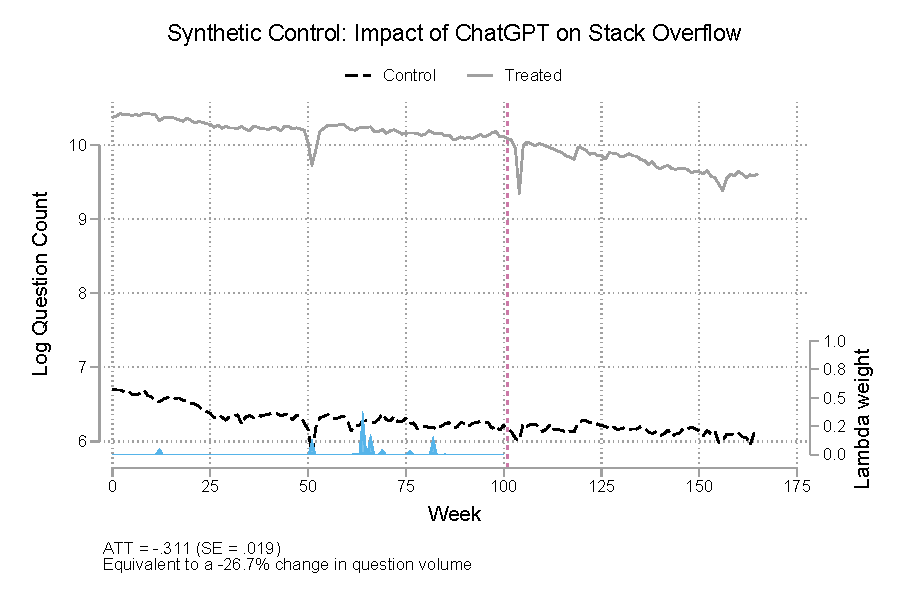
\includegraphics[width=1\textwidth]{imgs/stata/sdid_all_trends101.pdf}
        \caption{Impact on All Stack Overflow Questions}
        \label{fig:app-sdid_all}
    \end{subfigure}
    \hfill
    \begin{subfigure}[b]{0.475\textwidth}
        \centering
        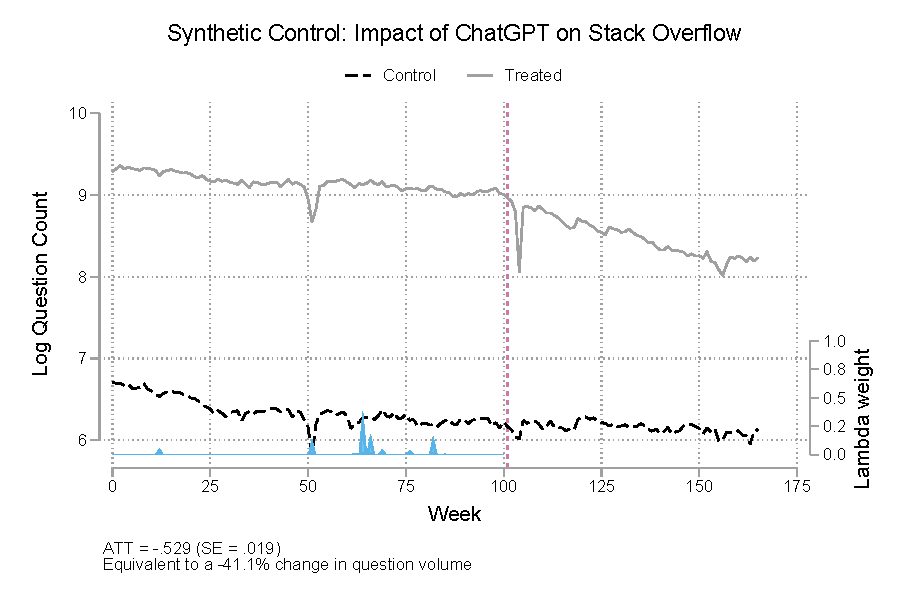
\includegraphics[width=1\textwidth]{imgs/stata/sdid_script_trends101.pdf}
        \caption{Impact on Scripting Language Questions}
        \label{fig:app-sdid_script}
    \end{subfigure}
    \caption{Synthetic difference-in-difference plots}
    \label{fig:app-DiD}
\end{figure}

\begin{table}[htpb!]
    \centering
    \caption{Synthetic DiD Estimates of ChatGPT's Impact on Stack Overflow Question Volume}
    \label{tab:app-sdid_results}
    \begin{tabular}{lcccc}
        \toprule
            & \multicolumn{2}{c}{All Questions} & \multicolumn{2}{c}{Scripting Languages} \\
            \cmidrule(lr){2-3} \cmidrule(lr){4-5}
            & (1) & (2) & (3) & (4) \\
        \midrule
            Treatment Effect & $-0.311^{***}$ & $-0.308^{***}$ & $-0.502^{***}$ & $-0.497^{***}$ \\
            & $(0.019)$ & $(0.000)$ & $(0.042)$ & $(0.039)$ \\
        \midrule
            Month covariates & No & Yes & No & Yes \\
            Percent Change & $-26.7\%$ & $-26.5\%$ & $-39.5\%$ & $-39.2\%$ \\
        \midrule
            Observations & 830 & 830 & 1,328 & 1,328 \\
            Number of groups & 5 & 5 & 8 & 8 \\
            Pre-treatment periods & 101 & 101 & 101 & 101 \\
            Post-treatment periods & 65 & 65 & 65 & 65 \\
        \bottomrule
            \multicolumn{5}{p{0.95\linewidth}}{\footnotesize \textit{Notes:} Standard errors in parentheses based on placebo/bootstrap replications (100 repetitions). $^{***}p<0.001$. The dependent variable is log question count. All models include time and group fixed effects. Treatment is defined as the period after ChatGPT's release (November 30, 2022).} \\
    \end{tabular}
\end{table}

%%%%%%%%%%%%%%%%%%%%%%%%%%%%%%%%%%%%%%%%%%%%%%%%%%%%%%%%%%%%%%%%%%%%%%%%%%%%%%%%%%%%%%%%%%%%%%%%

\begin{figure}[H]
    \centering
    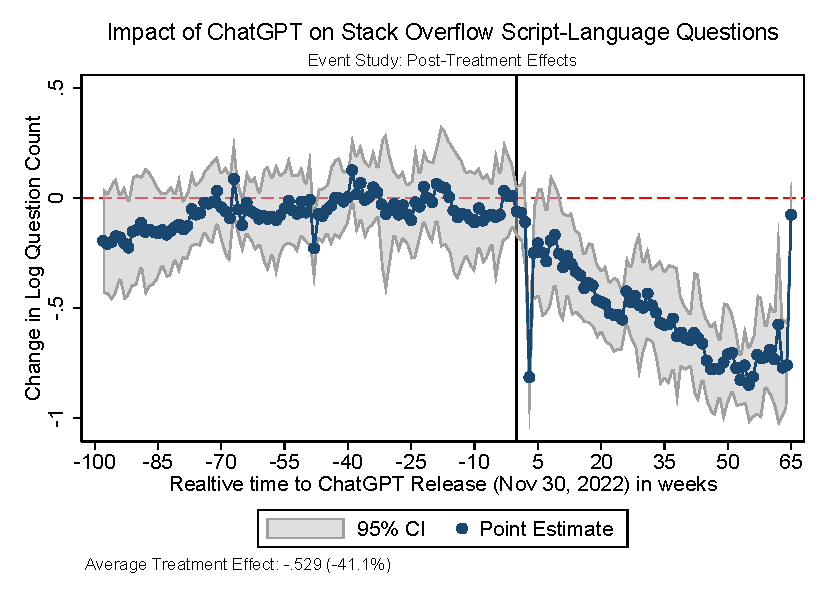
\includegraphics[width=0.9\textwidth]{imgs/stata/event_study_scripting_languages.pdf}
    \caption{Event Study Analysis for Scripting Language Questions}
    \label{fig:app-event_study}
\end{figure}

\begin{table}[H]
    \centering
    \caption{Event Study: Post-Treatment Effects Over Time for Scripting Languages}
    \label{tab:app-event_study_results}
    \begin{tabular}{lccc}
    \toprule
    Time Period & Estimate & SE & 95\% CI \\
    \midrule
    Week 1-4 after treatment   & -0.335 & 0.079 & [-0.490, -0.180] \\
    Week 5-12 after treatment  & -0.267 & 0.084 & [-0.432, -0.102] \\
    Week 13-24 after treatment & -0.482 & 0.080 & [-0.639, -0.325] \\
    Week 25-36 after treatment & -0.577 & 0.082 & [-0.738, -0.416] \\
    Week 37-48 after treatment & -0.644 & 0.077 & [-0.795, -0.493] \\
    Week 49-60 after treatment & -0.718 & 0.081 & [-0.877, -0.559] \\
    Week 61-65 after treatment & -0.739 & 0.077 & [-0.890, -0.588] \\
    \midrule
    Overall treatment effect & -0.502 & 0.073 & [-0.646, -0.358] \\
    \bottomrule
    \multicolumn{4}{p{0.95\linewidth}}{\footnotesize \textit{Notes:} Results from synthetic DiD event study analysis with bootstrapped standard errors (100 repetitions). Estimates show the change in log question count for Stack Overflow scripting language questions relative to the synthetic control group across different post-treatment time periods. All effects are statistically significant at the 0.1\% level.} \\
    \end{tabular}
\end{table}

%%%%%%%%%%%%%%%%%%%%%%%%%%%%%%%%%%%%%%%%%%%%%%%%%%%%%%%%%%%%%%%%%%%%%%%%%%%%%%%%%%%%%%%%%%%%%%%%

\section{Processing Pipeline}\label{app:procpipe}

\begin{figure}[H]
    \centering
    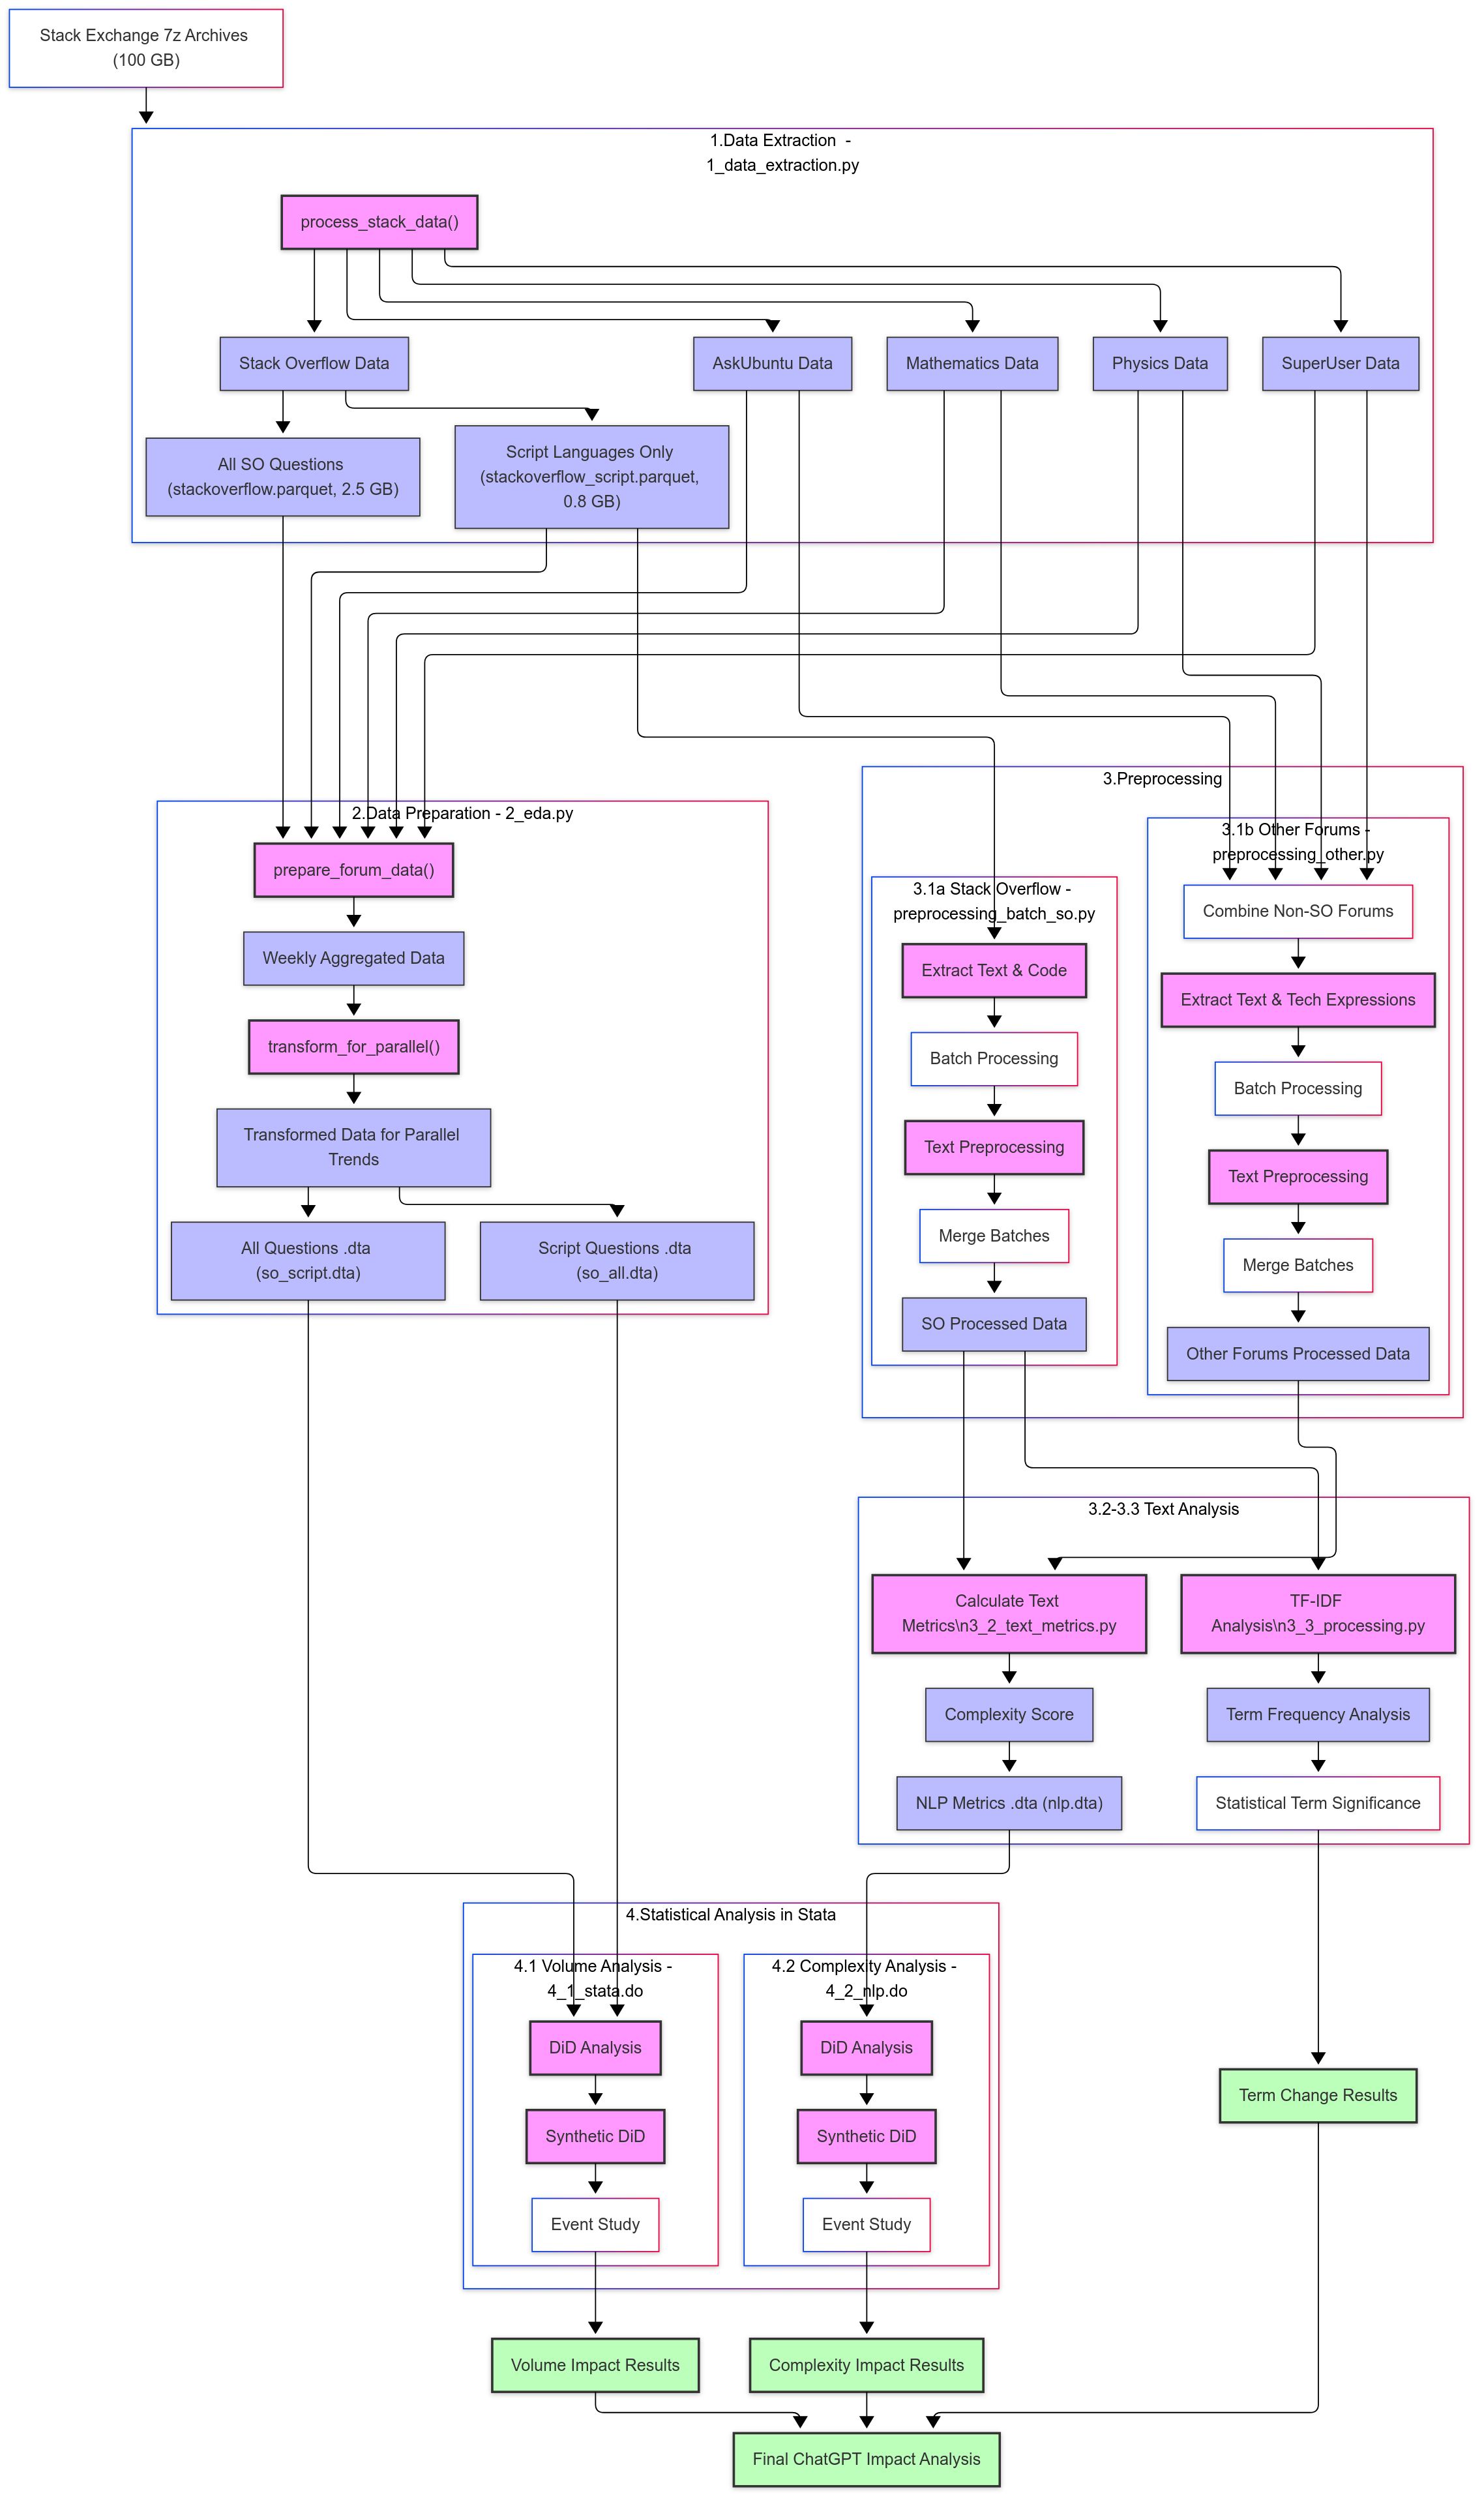
\includegraphics[width=0.8\linewidth]{imgs/process_flow.png}
    \caption{Sketched process and file flow}
    \label{fig:app-process_flow}
\end{figure}

%%%%%%%%%%%%%%%%%%%%%%%%%%%%%%%%%%%%%%%%%%%%%%%%%%%%%%%%%%%%%%%%%%%%%%%%%%%%%%%%%%%%%%%%%%%%%%%%

\section{Difference-in-Difference Complexity Scores}\label{app:didcs}

\begin{figure}[H]
    \centering
    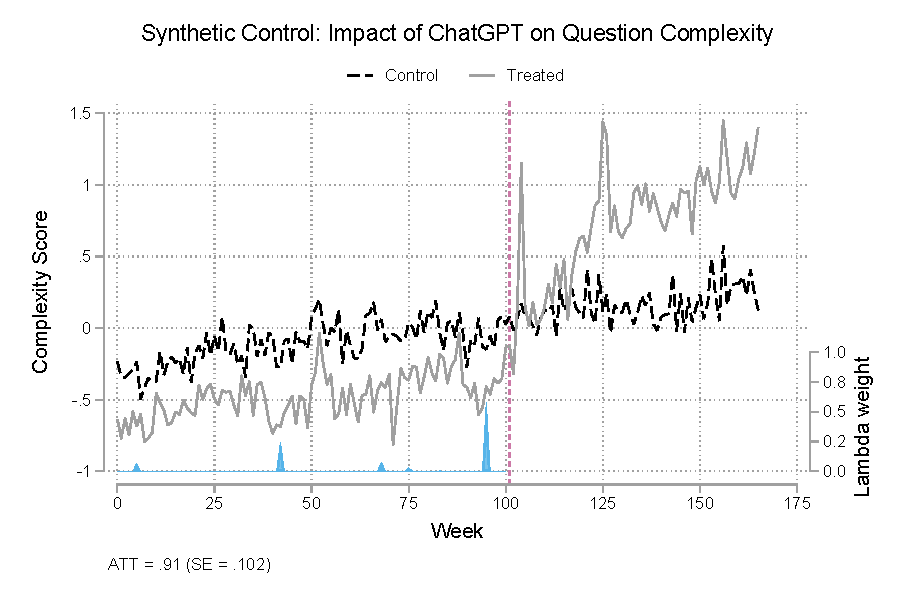
\includegraphics[width=1\linewidth]{imgs/stata/sdid_nlp_trends101.pdf}
    \caption{Synthetic DiD: Question complexity}
    \label{fig:app-cscore_synthetic_control}
\end{figure}

\begin{figure}[H]
    \centering
    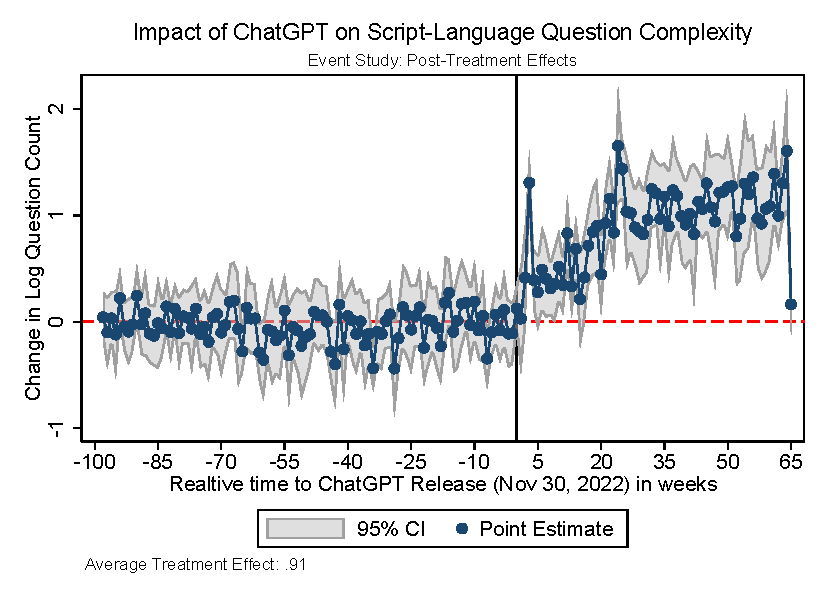
\includegraphics[width=1\linewidth]{imgs/stata/event_study_nlp.pdf}
    \caption{Event study complexity score development}
    \label{fig:app-cscore_event_study}
\end{figure}

\begin{table}[H]
    \centering
    \caption{Event Study: Post-Treatment Effects Over Time}
    \label{tab:app-csscore_event_study}
    \begin{tabular}{lccc}
    \toprule
    Time Period & Estimate & SE & 95\% CI \\
    \midrule
    Week 1-4 after treatment   & 0.016 & 0.025 & [-0.033, 0.065] \\
    Week 5-12 after treatment  & 0.028 & 0.022 & [-0.015, 0.071] \\
    Week 13-24 after treatment & 0.064 & 0.018 & [0.029, 0.099] \\
    Week 25-36 after treatment & 0.078 & 0.015 & [0.049, 0.107] \\
    Week 37-48 after treatment & 0.083 & 0.017 & [0.050, 0.116] \\
    Week 49-60 after treatment & 0.081 & 0.019 & [0.044, 0.118] \\
    Week 61-65 after treatment & 0.092 & 0.020 & [0.053, 0.131] \\
    \midrule
    Overall treatment effect & 0.059 & 0.014 & [0.032, 0.086] \\
    \bottomrule
    \multicolumn{4}{p{0.85\linewidth}}{\footnotesize \textit{Notes:} Results from synthetic DiD event study analysis. Estimates show the change in complexity score for Stack Overflow questions relative to the synthetic control group across different post-treatment time periods. Weeks 13-65 effects are statistically significant at the 5\% level, while the initial 1-12 week periods show positive but statistically insignificant effects.} \\
    \end{tabular}
\end{table}

\end{document}   